\chapter{DC Circuits: Kirchhoff's Laws and Theorems}\label{ch:b1:dc-circuits}

Turn the key on a cold morning: the starter groans, the dashboard lights
dim for a second, and the car coughs into life. The battery that
delivered a steady \qty{12.6}{V} a moment ago is down to eleven while
the starter draws its hundred and fifty \omterm{def:b1:dc-circuits:current}{amperes} --- and the headlights,
wired in parallel, pay for it. Everything in that second is governed by
two conservation laws and a handful of theorems about \omterm{def:b1:dc-circuits:linear}{linear circuits},
which this chapter states, proves, and applies: \omterm{thm:b1:dc-circuits:kirchhoff}{Kirchhoff's laws}, the
models of sources and \omterm{def:b1:dc-circuits:resistor}{resistors}, dividers, Thévenin and Norton, and
the graphical art of finding an \omterm{met:b1:dc-circuits:loadline}{operating point}.

\section{Current, voltage, and the quasi-steady regime}

\begin{definition}[Electric current]\label{def:b1:dc-circuits:current}
\index{electric current}\index{ampere}
The \emph{electric current} through a surface (a wire's cross-section)
is the charge crossing it per unit time, counted positively in a chosen
orientation:
\[
i = \frac{\dd q}{\dd t} \qquad (\text{amperes: } \qty{1}{A} = \qty{1}{C/s}).
\]
Reversing the orientation changes the sign of $i$. In a metal the
carriers are electrons, which drift \emph{against} the conventional
current direction, at a fraction of a millimeter per second.
\end{definition}

\begin{definition}[Potential and voltage]\label{def:b1:dc-circuits:voltage}
\index{electric potential}\index{voltage}\index{ground}
Each point of a circuit has an \emph{electric potential} $V$ (volts),
defined up to a constant fixed by choosing a \emph{ground} ($V = 0$).
The \emph{voltage} between $A$ and $B$ is the potential difference
$u_{AB} = V_A - V_B$, drawn as an arrow from $B$ to $A$. The energy a
charge $q$ loses in going from $A$ to $B$ is $q\,u_{AB}$ (this connects
to the electrostatic potential of \cref{ch:b1:potential-capacitors}).
\end{definition}

\begin{definition}[Quasi-steady regime (ARQS)]\label{def:b1:dc-circuits:arqs}
\index{quasi-steady regime}\index{ARQS}
A circuit of size $\ell$ driven at frequency $f$ is in the
\emph{quasi-steady regime} when the propagation time $\ell/c$ of
electrical \omterm{def:b1:wave-propagation:signal}{signals} along it is negligible against the period $1/f$:
$\ell \ll c/f$. The current is then the same at every point of an
unbranched wire at each instant, and the laws below apply at each
instant to time-varying currents and \omterm{def:b1:dc-circuits:voltage}{voltages} (lowercase $i$, $u$)
exactly as to steady ones ($I$, $U$).
\end{definition}

\begin{example}[How quasi is quasi]\label{ex:b1:dc-circuits:arqs}
At \qty{50}{Hz}, $c/f = \qty{6000}{km}$: a house is in the \omterm{def:b1:dc-circuits:arqs}{quasi-steady
regime}. At \qty{1}{MHz}, \qty{300}{m}: a radio still is. At \qty{2}{GHz},
\qty{15}{cm}: a phone's circuit board is not, and its tracks must be
treated as transmission lines --- a topic of the Year 2 volume.
\end{example}

\begin{theorem}[Kirchhoff's laws]\label{thm:b1:dc-circuits:kirchhoff}
\index{Kirchhoff's laws}\index{node law}\index{loop law}
In the \omterm{def:b1:dc-circuits:arqs}{quasi-steady regime}:
\begin{enumerate}
  \item \emph{\omterm{thm:b1:dc-circuits:kirchhoff}{Node law}}: at a node where several wires meet, the sum of
        the currents arriving equals the sum of the currents leaving,
        $\sum_{\text{in}} i_k = \sum_{\text{out}} i_k$.
  \item \emph{\omterm{thm:b1:dc-circuits:kirchhoff}{Loop law}}: around any closed loop, the \omterm{def:b1:dc-circuits:voltage}{voltages} add up to
        zero when counted with the sign given by a chosen direction of
        travel: $\sum_{\text{loop}} \pm u_k = 0$.
\end{enumerate}
\end{theorem}

\begin{proof}
Charge is conserved and, in the \omterm{def:b1:dc-circuits:arqs}{quasi-steady regime}, does not pile up
at a node: what arrives per second leaves per second. The \omterm{thm:b1:dc-circuits:kirchhoff}{loop law} is
the statement that the potential is a function of position: going
around a loop and back to the starting point, the sum of the potential
drops is $V_A - V_A = 0$.
\end{proof}

\begin{notation}[Conventions and power]\label{not:b1:dc-circuits:conventions}
\index{receiver convention}\index{generator convention}\index{electric power}
For a two-terminal component (a \emph{dipole}), the \emph{\omterm{thm:b1:dc-circuits:kirchhoff}{receiver
convention}} draws the \omterm{def:b1:dc-circuits:voltage}{voltage} arrow and the current arrow in opposite
directions; the \emph{\omterm{thm:b1:dc-circuits:kirchhoff}{generator convention}} draws them in the same
direction. In the \omterm{thm:b1:dc-circuits:kirchhoff}{receiver convention}, the power \emph{received} by the
dipole is
\[
p = u\,i \qquad (\text{watts}),
\]
positive for a \omterm{def:b1:dc-circuits:resistor}{resistor} that heats, negative for a battery that
delivers. In the \omterm{thm:b1:dc-circuits:kirchhoff}{generator convention} $p = ui$ is the power
\emph{delivered}.
\end{notation}

\begin{omfigure}
\begin{tikzpicture}[font=\small]
  \draw (0,0) to[generic, l=dipole, v=$u$, i=$i$] (3,0);
  \node[below] at (1.5,-1.0) {receiver convention: $p_{\text{received}} = ui$};
  \begin{scope}[xshift=6cm]
  \draw (0,0) to[generic, l=dipole, v<=$u$, i=$i$] (3,0);
  \node[below] at (1.5,-1.0) {generator convention: $p_{\text{delivered}} = ui$};
  \end{scope}
\end{tikzpicture}

{\small The two sign conventions for a dipole: arrows opposed
(receiver) or aligned (generator). The physics is the same; only the
sign of $ui$ is read differently.}
\end{omfigure}

\section{Dipoles and their models}

\begin{definition}[Characteristic; resistor; Ohm's law]\label{def:b1:dc-circuits:resistor}
\index{characteristic (of a dipole)}\index{resistor}\index{Ohm's law}\index{Joule effect}
The \emph{characteristic} of a dipole is the curve $i(u)$ (or $u(i)$)
it imposes. A \emph{resistor} has a linear characteristic through the
origin, \emph{Ohm's law}
\[
u = R\,i \qquad (\text{receiver convention}),
\]
$R$ being its \emph{resistance} (ohms, $\qty{1}{\ohm} = \qty{1}{V/A}$) and
$G = 1/R$ its \emph{conductance} (siemens). It receives $p = Ri^2 =
u^2/R \geq 0$, dissipated as heat (\emph{Joule effect}). A wire of
length $\ell$, cross-section $S$ and resistivity $\rho$ has
$R = \rho\ell/S$.
\end{definition}

\begin{definition}[Ideal and real sources]\label{def:b1:dc-circuits:sources}
\index{voltage source}\index{current source}\index{electromotive force}\index{internal resistance}\index{Thevenin model@Thévenin model}\index{Norton model}
An \emph{ideal \omterm{def:b1:dc-circuits:voltage}{voltage} source} imposes $u = E$ whatever the current;
$E$ is its \emph{electromotive force} (emf). An \emph{ideal current
source} imposes $i = I_N$ whatever the \omterm{def:b1:dc-circuits:voltage}{voltage}. A \emph{real source}
(battery, generator, power supply) is modeled, in the \omterm{thm:b1:dc-circuits:kirchhoff}{generator
convention}, by
\[
u = E - r\,i \quad (\text{Thévenin model: ideal emf } E \text{ in series with } r)
\]
or, equivalently, by $i = I_N - u/r$ (Norton model: ideal current
source $I_N = E/r$ in parallel with $r$); $r$ is the \emph{internal
resistance}. $E$ is the open-circuit \omterm{def:b1:dc-circuits:voltage}{voltage}, $I_N = E/r$ the
short-circuit current.
\end{definition}

\begin{proposition}[Power balance of a real source]\label{prop:b1:dc-circuits:sourcepower}
\index{maximum power transfer}
A real source $(E, r)$ feeding a \omterm{def:b1:dc-circuits:resistor}{resistor} $R$ delivers $i = E/(R + r)$
and the power
\[
P_R = \frac{E^2 R}{(R + r)^2},
\]
maximal and equal to $E^2/4r$ when $R = r$ (\emph{impedance matching}),
with efficiency $P_R/(Ei) = R/(R + r)$, only $50\%$ at the maximum.
\end{proposition}

\begin{proof}
\omterm{thm:b1:dc-circuits:kirchhoff}{Loop law}: $E = ri + Ri$. $P_R = Ri^2$; differentiate $R/(R + r)^2$:
$\big[(R + r)^2 - 2R(R + r)\big]/(R + r)^4 = (r - R)/(R + r)^3$, zero at
$R = r$, positive before and negative after. The source supplies
$Ei = (R + r)i^2$, of which $ri^2$ heats the source itself.
\end{proof}

\begin{omfigure}
\begin{tikzpicture}
\begin{axis}[omaxis, width=7.6cm, height=5.2cm, xlabel={$i$}, ylabel={$u$},
    xmin=0, xmax=1.3, ymin=0, ymax=1.3, xtick={1}, xticklabels={$I_N = E/r$},
    ytick={1}, yticklabels={$E$}]
  \addplot[omThm, thick, domain=0:1, samples=2] {1 - x};
  \addplot[omDef, thick, domain=0:0.9, samples=2] {0.6*x};
  \fill[omExo] (axis cs:0.625,0.375) circle (1.6pt);
  \node[omExo, font=\footnotesize] (op) at (axis cs:0.98,0.92) {operating point};
  \draw[-Stealth, omExo] (op.south west) -- (axis cs:0.645,0.395);
  \node[omThm, font=\footnotesize, anchor=south west] at (axis cs:0.03,1.02) {source $u = E - ri$};
  \node[omDef, font=\footnotesize, right] at (axis cs:0.9,0.54) {load $u = Ri$};
\end{axis}
\end{tikzpicture}\qquad
\begin{tikzpicture}
\begin{axis}[omaxis, width=7.0cm, height=5cm, xlabel={$R/r$}, ylabel={$P_R$},
    xmin=0, xmax=6, ymin=0, ymax=0.3, xtick={1,3,5}, ytick={0.25}, yticklabels={$\frac{E^2}{4r}$}]
  \addplot[omProp, thick, domain=0:6, samples=120] {x/((x+1)^2)};
  \draw[dashed, omExo] (axis cs:1,0) -- (axis cs:1,0.25) -- (axis cs:0,0.25);
\end{axis}
\end{tikzpicture}

{\small Left: the characteristics of a real source ($u = E - ri$) and
of a resistive load ($u = Ri$) meet at the \omterm{met:b1:dc-circuits:loadline}{operating point}. Right: the
power delivered to the load peaks at $R = r$, where half of the source's
power is wasted in its own resistance.}
\end{omfigure}

\begin{example}[A car battery under load]\label{ex:b1:dc-circuits:battery}
Open circuit \qty{12.6}{V}; \qty{11.4}{V} while the starter draws
\qty{120}{A}: $r = 1.2/120 = \qty{10}{m\ohm}$, $I_N = \qty{1260}{A}$
(hence the welding-grade danger of a dropped spanner). Matched load
$R = \qty{10}{m\ohm}$ would take $E^2/4r = \qty{4}{kW}$ for a few
seconds --- about what a starter motor needs.
\end{example}

\begin{remark}[Other dipoles]\label{rem:b1:dc-circuits:others}
\index{diode}
A \emph{diode} conducts in one direction only: an idealized model is an
open circuit for $u < U_0$ and a fixed \omterm{def:b1:dc-circuits:voltage}{voltage} $u = U_0$ (about
\qty{0.7}{V} for silicon, \qty{2}{} to \qty{3}{V} for an LED) when it
conducts. A filament lamp is a \omterm{def:b1:dc-circuits:resistor}{resistor} whose $R$ grows with its
temperature, hence with $i$ --- a curved characteristic. In steady
state a capacitor is an open circuit ($i = C\,\dd u/\dd t = 0$) and an
inductor a short circuit ($u = L\,\dd i/\dd t = 0$); their role in
transients is \cref{ch:b1:transient-regimes}.
\end{remark}

\section{Associations and dividers}

\begin{proposition}[Series and parallel resistors]\label{prop:b1:dc-circuits:seriesparallel}
\index{series (resistors)}\index{parallel (resistors)}
\omterm{def:b1:dc-circuits:resistor}{Resistors} in series (same current) add: $R = R_1 + R_2 + \cdots$.
\omterm{def:b1:dc-circuits:resistor}{Resistors} in parallel (same \omterm{def:b1:dc-circuits:voltage}{voltage}) add their conductances:
$1/R = 1/R_1 + 1/R_2 + \cdots$; for two, $R = R_1R_2/(R_1 + R_2)$,
written $R_1 \parallel R_2$.
\end{proposition}

\begin{proof}
Series: $u = u_1 + u_2 = (R_1 + R_2)i$ (\omterm{thm:b1:dc-circuits:kirchhoff}{loop law}). Parallel: $i = i_1 +
i_2 = u/R_1 + u/R_2$ (\omterm{thm:b1:dc-circuits:kirchhoff}{node law}).
\end{proof}

\begin{proposition}[Voltage and current dividers]\label{prop:b1:dc-circuits:dividers}
\index{voltage divider}\index{current divider}
Two \omterm{def:b1:dc-circuits:resistor}{resistors} in series across a \omterm{def:b1:dc-circuits:voltage}{voltage} $u$ share it in proportion to
their resistances:
\[
u_2 = \frac{R_2}{R_1 + R_2}\,u .
\]
Two \omterm{def:b1:dc-circuits:resistor}{resistors} in parallel fed by a current $i$ share it in inverse
proportion:
\[
i_2 = \frac{R_1}{R_1 + R_2}\,i = \frac{G_2}{G_1 + G_2}\,i .
\]
\end{proposition}

\begin{proof}
Series: $i = u/(R_1 + R_2)$ and $u_2 = R_2 i$. Parallel: $u = (R_1
\parallel R_2)\,i$ and $i_2 = u/R_2$.
\end{proof}

\begin{omfigure}
\begin{tikzpicture}[font=\small]
  \draw (0,3.2) to[R=$R_1$] (0,1.6) to[R=$R_2$, v=$u_2$] (0,0);
  \draw[-Stealth, thick] (-1.3,0.1) -- (-1.3,3.1) node[midway, left] {$u$};
  \fill (0,3.2) circle (1.2pt); \fill (0,0) circle (1.2pt);
  \begin{scope}[xshift=5.5cm]
  \draw (0,3.2) to[short, i=$i$] (1.4,3.2) to[R=$R_1$] (1.4,0) -- (0,0);
  \draw (1.4,3.2) -- (3.0,3.2) to[short, i=$i_2$] (3.0,2.4) to[R=$R_2$] (3.0,0) -- (1.4,0);
  \fill (0,3.2) circle (1.2pt); \fill (0,0) circle (1.2pt);
  \end{scope}
\end{tikzpicture}

{\small \omterm{prop:b1:dc-circuits:dividers}{Voltage divider} (left): $u_2 = R_2 u/(R_1 + R_2)$. \omterm{prop:b1:dc-circuits:dividers}{Current
divider} (right): $i_2 = R_1 i/(R_1 + R_2)$ --- the current prefers the
smaller resistance.}
\end{omfigure}

\begin{remark}[Loading a divider]\label{rem:b1:dc-circuits:loading}
The divider formula holds only if nothing draws current from the
midpoint. A load $R_L$ connected across $R_2$ replaces $R_2$ by $R_2
\parallel R_L$ and lowers $u_2$ --- the ``loading effect'', and the
reason a voltmeter must have a high resistance and a potentiometer a
low one compared with what it feeds
(\cref{exo:b1:dc-circuits:4}).
\end{remark}

\begin{method}[Reducing a network]\label{met:b1:dc-circuits:reduce}
To find one current or \omterm{def:b1:dc-circuits:voltage}{voltage} in a network of \omterm{def:b1:dc-circuits:resistor}{resistors} and one
source:
\begin{enumerate}
  \item starting far from the source, replace series and parallel
        groups by their equivalents until a single \omterm{def:b1:dc-circuits:resistor}{resistor} faces the
        source;
  \item compute the source current;
  \item walk back, splitting currents with \omterm{prop:b1:dc-circuits:dividers}{current dividers} and
        \omterm{def:b1:dc-circuits:voltage}{voltages} with \omterm{prop:b1:dc-circuits:dividers}{voltage dividers}, down to the wanted branch.
\end{enumerate}
With several sources, or for a branch whose neighbors change, use the
theorems of the next section.
\end{method}

\section{Theorems for linear circuits}

\begin{definition}[Linear dipole, linear circuit]\label{def:b1:dc-circuits:linear}
\index{linear dipole}
A dipole is \emph{linear} if its characteristic is a straight line
(\omterm{def:b1:dc-circuits:resistor}{resistor}, ideal and real sources); a circuit made only of linear
dipoles is a \emph{linear circuit}. Its unknowns obey a system of
linear equations (\omterm{thm:b1:dc-circuits:kirchhoff}{Kirchhoff's laws} plus the characteristics), whose
solution is unique.
\end{definition}

\begin{theorem}[Thévenin and Norton]\label{thm:b1:dc-circuits:thevenin}
\index{Thevenin's theorem@Thévenin's theorem}\index{Norton's theorem}
Seen from two of its terminals $A$ and $B$, any \omterm{def:b1:dc-circuits:linear}{linear circuit} is
equivalent to a real source: an emf $E_{\mathrm{Th}}$ in series with a
resistance $R_{\mathrm{Th}}$ (Thévenin), or a \omterm{def:b1:dc-circuits:sources}{current source} $I_N =
E_{\mathrm{Th}}/R_{\mathrm{Th}}$ in parallel with $R_{\mathrm{Th}}$
(Norton), where
\begin{itemize}
  \item $E_{\mathrm{Th}}$ is the open-circuit \omterm{def:b1:dc-circuits:voltage}{voltage} $u_{AB}$;
  \item $I_N$ is the short-circuit current from $A$ to $B$;
  \item $R_{\mathrm{Th}}$ is the resistance seen between $A$ and $B$
        when every independent source is switched off (ideal \omterm{def:b1:dc-circuits:sources}{voltage
        sources} replaced by wires, ideal \omterm{def:b1:dc-circuits:sources}{current sources} by open
        circuits).
\end{itemize}
\end{theorem}

\begin{proof}[Partial proof]
By linearity, the relation between the \omterm{def:b1:dc-circuits:voltage}{voltage} $u_{AB}$ and the current
$i$ drawn at the terminals is affine: $u_{AB} = a - b\,i$. Setting
$i = 0$ identifies $a = E_{\mathrm{Th}}$; setting $u_{AB} = 0$ gives
$b = E_{\mathrm{Th}}/I_N$. That $b$ equals the resistance seen with
sources killed follows from superposition (below): the part of $u_{AB}$
due to the external current alone is what a passive network of
resistance $R_{\mathrm{Th}}$ would produce. That every linear system has
an affine input--output relation is the algebra of linear equations.
\end{proof}

\begin{theorem}[Superposition]\label{thm:b1:dc-circuits:superposition}
\index{superposition theorem}
In a \omterm{def:b1:dc-circuits:linear}{linear circuit} with several independent sources, any current or
\omterm{def:b1:dc-circuits:voltage}{voltage} is the sum of the values it takes when each source acts alone,
the others being switched off.
\end{theorem}

\begin{proof}
The equations are linear in the unknowns, with the sources as the
right-hand side; the solution is a linear function of that right-hand
side, hence the sum of the solutions for each source separately.
\end{proof}

\begin{proposition}[Millman's theorem]\label{prop:b1:dc-circuits:millman}
\index{Millman's theorem}
A node $N$ connected to points of potentials $V_1, \dots, V_n$ through
resistances $R_1, \dots, R_n$ (and to nothing else) has the potential
\[
V_N = \frac{\sum_k V_k/R_k}{\sum_k 1/R_k} = \frac{\sum_k G_k V_k}{\sum_k G_k},
\]
the conductance-weighted mean of its neighbors' potentials.
\end{proposition}

\begin{proof}
\omterm{thm:b1:dc-circuits:kirchhoff}{Node law} at $N$: $\sum_k (V_k - V_N)/R_k = 0$; solve for $V_N$.
\end{proof}

\begin{omfigure}
\begin{tikzpicture}[font=\small]
  % network: E1=10V, R1=1k ; E2=5V, R2=2k ; common load R3=2k
  \draw (0,0) to[battery1, l=$E_1$, invert] (0,2) to[R=$R_1$] (2.5,2) -- (2.5,2) to[R=$R_3$, v=$u$] (2.5,0) -- (0,0);
  \draw (2.5,2) to[R=$R_2$] (5,2) to[battery1, l_=$E_2$] (5,0) -- (2.5,0);
  \node at (2.5,2.45) {$N$};
  \node at (6.4,1) {$\Longleftrightarrow$};
  \begin{scope}[xshift=8.8cm]
  \draw (0,0) to[battery1, l=$E_{\mathrm{Th}}$, invert] (0,2) to[R=$R_{\mathrm{Th}}$] (2.2,2) to[R=$R_3$, v=$u$] (2.2,0) -- (0,0);
  \end{scope}
\end{tikzpicture}

{\small Two sources feeding a common load $R_3$. Seen from $R_3$'s
terminals, the rest of the circuit is a Thévenin source
($E_{\mathrm{Th}}$, $R_{\mathrm{Th}}$); Millman's theorem gives the
potential of node $N$ in one line.}
\end{omfigure}

\begin{example}[Three ways to the same answer]\label{ex:b1:dc-circuits:threeways}
In the figure, $E_1 = \qty{10}{V}$, $R_1 = \qty{1.0}{k\ohm}$, $E_2 =
\qty{5.0}{V}$, $R_2 = \qty{2.0}{k\ohm}$, $R_3 = \qty{2.0}{k\ohm}$.
\emph{Millman}: $V_N = (10/1 + 5/2 + 0/2)/(1 + 0.5 + 0.5) = 12.5/2 =
\qty{6.25}{V}$. \emph{Superposition}: $E_1$ alone sees $R_2 \parallel
R_3 = \qty{1}{k\ohm}$, so $u = 10 \times 1/2 = \qty{5}{V}$; $E_2$ alone
sees $R_1 \parallel R_3 = \qty{0.667}{k\ohm}$, $u = 5 \times 0.667/2.667
= \qty{1.25}{V}$; total \qty{6.25}{V}. \emph{Thévenin} seen from
$R_3$: $E_{\mathrm{Th}}$ is the open-circuit \omterm{def:b1:dc-circuits:voltage}{voltage} of the divider
$(E_1, R_1, R_2, E_2)$: $E_2 + (E_1 - E_2)R_2/(R_1 + R_2) = 5 + 5 \times
2/3 = \qty{8.33}{V}$; $R_{\mathrm{Th}} = R_1 \parallel R_2 =
\qty{0.667}{k\ohm}$; then $u = 8.33 \times 2/2.667 = \qty{6.25}{V}$.
\end{example}

\section{Operating point; the Wheatstone bridge}

\begin{method}[Graphical operating point]\label{met:b1:dc-circuits:loadline}
\index{operating point}\index{load line}
A non-linear dipole (characteristic $i = g(u)$) fed by a Thévenin
source $(E, R)$ settles where both relations hold: draw the dipole's
characteristic and the source's \emph{\omterm{met:b1:dc-circuits:loadline}{load line}} $u = E - Ri$ on the
same axes; their intersection is the \emph{\omterm{met:b1:dc-circuits:loadline}{operating point}}. Designing
the series \omterm{def:b1:dc-circuits:resistor}{resistor} of an LED, a Zener regulator or a transistor's bias
is exactly this construction.
\end{method}

\begin{omfigure}
\begin{tikzpicture}
\begin{axis}[omaxis, width=8cm, height=5.4cm, xlabel={$u$ (\unit{V})}, ylabel={$i$ (\unit{mA})},
    xmin=0, xmax=5.6, ymin=0, ymax=30, xtick={1,2,3,4,5}, ytick={10,20,25}]
  \addplot[omDef, thick, domain=0:1.9, samples=2] {0};
  \addplot[omDef, thick, domain=1.9:2.9, samples=60] {28*(exp(2.8*(x-1.9))-1)/(exp(2.8)-1)};
  \addplot[omThm, thick, domain=0:5, samples=2] {25 - 5*x};
  \fill[omExo] (axis cs:2.0,15) circle (1.6pt);
  \node[omExo, font=\footnotesize] (op) at (axis cs:1.05,11.5) {operating point};
  \draw[-Stealth, omExo] (op.east) -- (axis cs:1.93,14.8);
  \node[omDef, font=\footnotesize, left] at (axis cs:2.55,25) {LED};
  \node[omThm, font=\footnotesize] at (axis cs:3.1,1.4) {load line};
\end{axis}
\end{tikzpicture}

{\small An LED (threshold near \qty{2}{V}) fed by $E = \qty{5}{V}$
through $R = \qty{200}{\ohm}$: the \omterm{met:b1:dc-circuits:loadline}{load line} $u = E - Ri$ crosses the
diode's characteristic at $\qty{2.0}{V}$, \qty{15}{mA}. Raising $R$
tilts the line down and dims the LED.}
\end{omfigure}

\begin{proposition}[Wheatstone bridge]\label{prop:b1:dc-circuits:wheatstone}
\index{Wheatstone bridge}
Four \omterm{def:b1:dc-circuits:resistor}{resistors} $R_1, R_2$ (one branch) and $R_3, R_4$ (the other) across
a source $E$; the bridge output is the \omterm{def:b1:dc-circuits:voltage}{voltage} between the two
midpoints:
\[
u = E\left(\frac{R_2}{R_1 + R_2} - \frac{R_4}{R_3 + R_4}\right),
\]
zero (the bridge is \emph{balanced}) iff $R_1R_4 = R_2R_3$. For a
balanced bridge with $R_4$ perturbed to $R_4(1 + \epsilon)$, $\epsilon
\ll 1$, and $R_3 = R_4$: $u \approx -E\epsilon/4$.
\end{proposition}

\begin{proof}
Two \omterm{prop:b1:dc-circuits:dividers}{voltage dividers}; subtract. Balance: $R_2(R_3 + R_4) = R_4(R_1 +
R_2)$, i.e.\ $R_2R_3 = R_1R_4$. With $R_3 = R_4 = R$ and $R_1 = R_2$:
$u = E[\tfrac12 - (1 + \epsilon)/(2 + \epsilon)] = E[(2 + \epsilon - 2 -
2\epsilon)/(2(2 + \epsilon))] \approx -E\epsilon/4$.
\end{proof}

\begin{omfigure}
\begin{tikzpicture}[font=\small]
  \draw (0,1.5) to[R=$R_1$] (2,3) to[R=$R_2$] (4,1.5) to[R=$R_4$] (2,0) to[R=$R_3$] (0,1.5);
  \draw (2,3) to[short, *-] (2,3); \draw (2,0) to[short, *-] (2,0);
  \draw (0,1.5) -- (-1,1.5) to[battery1, l=$E$] (-1,-1) -- (4,-1) -- (4,1.5);
  \draw[-Stealth, omThm] (2,0.35) -- (2,2.65) ;
  \node[omThm, right] at (2.05,1.5) {$u$};
\end{tikzpicture}

{\small The \omterm{prop:b1:dc-circuits:wheatstone}{Wheatstone bridge}: two dividers side by side. Balanced when
$R_1R_4 = R_2R_3$, it converts a tiny change of one resistance
(strain gauge, thermistor) into a \omterm{def:b1:dc-circuits:voltage}{voltage} around zero, which is far
easier to amplify than a small change of a large \omterm{def:b1:dc-circuits:voltage}{voltage}.}
\end{omfigure}

\section{Exercises}

\begin{exercise}[$\star$]\label{exo:b1:dc-circuits:1}
A phone charges at \qty{1.5}{A} for one hour: what charge flows, how
many electrons? Estimate whether the \omterm{def:b1:dc-circuits:arqs}{quasi-steady regime} holds for the
house wiring at \qty{50}{Hz}, for a \qty{10}{cm} circuit at \qty{1}{MHz},
and for the same circuit at \qty{1}{GHz}.
\end{exercise}

\begin{exercise}[$\star$]\label{exo:b1:dc-circuits:2}
A \qty{2000}{W} heater on \qty{230}{V}: current, resistance, energy
used in \qty{3.0}{h} (in kWh and in joules). Its \qty{5.0}{m} copper
cord has a cross-section of \qty{1.5}{mm^2} ($\rho = \qty{1.7e-8}{\ohm.m}$):
power lost in the cord.
\end{exercise}

\begin{exercise}[$\star$]\label{exo:b1:dc-circuits:3}
With $\qty{10}{\ohm}$, $\qty{20}{\ohm}$ and $\qty{30}{\ohm}$: compute
the resistance of the three in series, in parallel, and of
$(10 \parallel 20) + 30$.
\end{exercise}

\begin{exercise}[$\star$]\label{exo:b1:dc-circuits:4}
A \qty{12}{V} source feeds \qty{4.7}{k\ohm} and \qty{2.2}{k\ohm} in
series. Compute the \omterm{def:b1:dc-circuits:voltage}{voltage} across the \qty{2.2}{k\ohm}. A device of
resistance \qty{2.2}{k\ohm} is then connected across it: new \omterm{def:b1:dc-circuits:voltage}{voltage}?
Conclude on the loading effect.
\end{exercise}

\begin{exercise}[$\star\star$]\label{exo:b1:dc-circuits:5}
A battery reads \qty{12.6}{V} open and \qty{11.4}{V} while delivering
\qty{120}{A}. Find its \omterm{def:b1:dc-circuits:sources}{internal resistance} and short-circuit current,
the power delivered to the starter and the power lost inside, and the
efficiency.
\end{exercise}

\begin{exercise}[$\star\star$]\label{exo:b1:dc-circuits:6}
Find the Thévenin equivalent, seen from the \qty{2.2}{k\ohm}
\omterm{def:b1:dc-circuits:resistor}{resistor}'s terminals, of the divider of \cref{exo:b1:dc-circuits:4}
($E = \qty{12}{V}$, $R_1 = \qty{4.7}{k\ohm}$, $R_2 = \qty{2.2}{k\ohm}$).
Use it to recover the loaded \omterm{def:b1:dc-circuits:voltage}{voltage} of that exercise.
\end{exercise}

\begin{exercise}[$\star\star$]\label{exo:b1:dc-circuits:7}
Two batteries, $E_1 = \qty{10}{V}$ ($r_1 = \qty{1.0}{\ohm}$) and
$E_2 = \qty{5.0}{V}$ ($r_2 = \qty{2.0}{\ohm}$), are connected in
parallel (same polarity) across a \qty{2.0}{\ohm} load. Find the load
\omterm{def:b1:dc-circuits:voltage}{voltage} by superposition, then by Millman, and the current in each
battery. Is the weaker battery charging or discharging?
\end{exercise}

\begin{exercise}[$\star\star$]\label{exo:b1:dc-circuits:8}
A source $E = \qty{9.0}{V}$, $r = \qty{3.0}{\ohm}$. Compute the power
delivered to loads of $\qty{1.0}{\ohm}$, $\qty{3.0}{\ohm}$, $\qty{12}{\ohm}$,
and the efficiency in each case. Which load would an engineer choose for
a battery-powered device, and why not the matched one?
\end{exercise}

\begin{exercise}[$\star\star$]\label{exo:b1:dc-circuits:9}
An LED conducts at \qty{2.0}{V} and must carry \qty{15}{mA} from a
\qty{5.0}{V} supply. Choose the series \omterm{def:b1:dc-circuits:resistor}{resistor}, the powers in the
\omterm{def:b1:dc-circuits:resistor}{resistor} and in the LED, and sketch the \omterm{met:b1:dc-circuits:loadline}{load line} construction. What
happens if the supply is \qty{3.3}{V}?
\end{exercise}

\begin{exercise}[$\star\star\star$]\label{exo:b1:dc-circuits:10}
A strain gauge $R_4 = R(1 + \epsilon)$, $R = \qty{1.0}{k\ohm}$, sits in a
\omterm{prop:b1:dc-circuits:wheatstone}{Wheatstone bridge} with three fixed \qty{1.0}{k\ohm} \omterm{def:b1:dc-circuits:resistor}{resistors} across
\qty{5.0}{V}. Derive the output \omterm{def:b1:dc-circuits:voltage}{voltage} to first order in $\epsilon$ and
compute it for $\epsilon = \num{1.0e-3}$. Why is the bridge preferable
to measuring the gauge's \omterm{def:b1:dc-circuits:voltage}{voltage} in a simple divider?
\end{exercise}

\begin{exercise}[$\star\star\star$]\label{exo:b1:dc-circuits:11}
Twelve identical \omterm{def:b1:dc-circuits:resistor}{resistors} $R$ form the edges of a cube. Using
symmetry (which nodes are at the same potential when a current $I$
enters one corner and leaves the opposite one), show that the
resistance between opposite corners is $5R/6$.
\end{exercise}

\begin{exercise}[$\star\star\star$]\label{exo:b1:dc-circuits:12}
A \omterm{def:b1:dc-circuits:sources}{current source} $I_N = \qty{2.0}{A}$ in parallel with \qty{4.0}{\ohm}
is connected, through a \qty{2.0}{\ohm} \omterm{def:b1:dc-circuits:resistor}{resistor}, to a \qty{6.0}{V}
battery (negligible resistance) whose emf opposes it. Convert the
Norton source to Thévenin and find the current in the \qty{2.0}{\ohm}
\omterm{def:b1:dc-circuits:resistor}{resistor} and the power exchanged by each source.
\end{exercise}

\begin{omfigure}
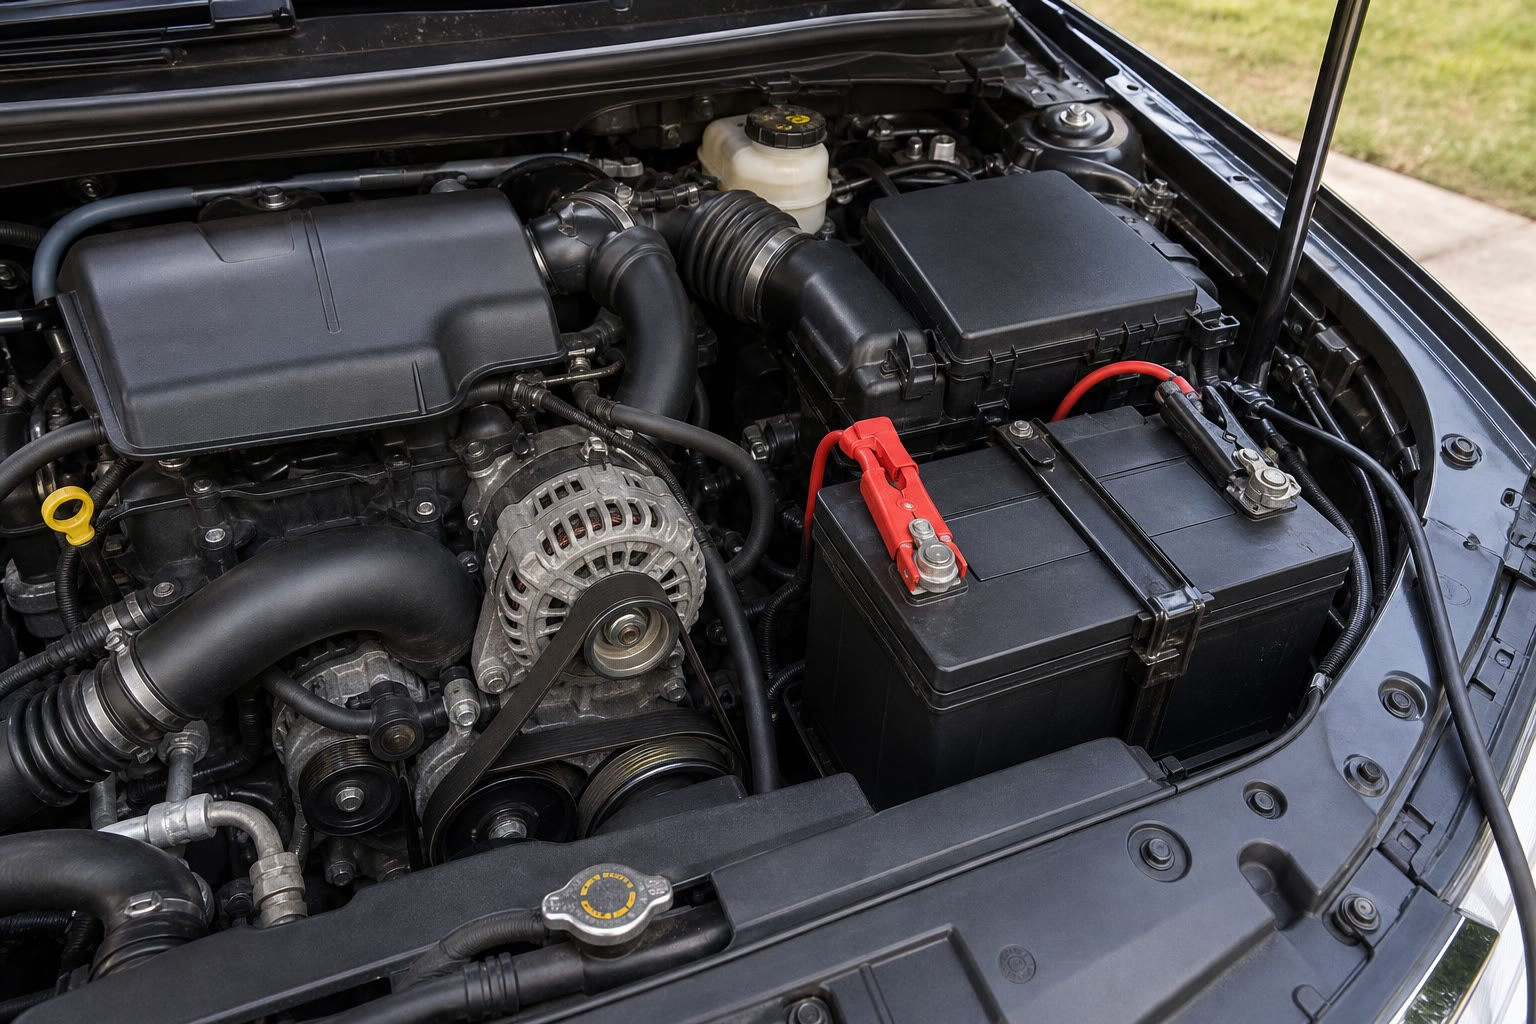
\includegraphics[width=0.58\linewidth]{images/book3/ai/b3-06-car-battery-engine-bay.jpg}

{\small Under the bonnet: the \qty{12}{V} battery, its thick cables and the alternator --- the direct-current network of the weekend problem, with hundreds of \omterm{def:b1:dc-circuits:current}{amperes} at start-up.}
\end{omfigure}

\section{Problem: A car's electrical system}

\begin{problem}[{Weekend problem --- one battery, a starter, two
headlights, an alternator and a few meters of copper: who gets the
current, who pays, and why the lights dim when the engine cranks}]
\label{pb:b1:dc-circuits:1}
The battery is a real source, emf $E = \qty{12.6}{V}$, \omterm{def:b1:dc-circuits:sources}{internal
resistance} $r = \qty{10}{m\ohm}$. Copper: $\rho = \qty{1.7e-8}{\ohm.m}$.

\medskip
\noindent\textbf{Part I --- The battery alone.}
\begin{enumerate}
  \item Draw the \omterm{def:b1:dc-circuits:sources}{Thévenin model} and write $u(i)$ in the \omterm{thm:b1:dc-circuits:kirchhoff}{generator
        convention}.
  \item Give the open-circuit \omterm{def:b1:dc-circuits:voltage}{voltage} and the short-circuit current.
        Why must a dropped wrench never bridge the terminals?
  \item Write the \omterm{def:b1:dc-circuits:sources}{Norton model} of the same battery.
  \item The battery feeds a \omterm{def:b1:dc-circuits:resistor}{resistor} $R$: express the current, the
        terminal \omterm{def:b1:dc-circuits:voltage}{voltage}, the power $P_R$ delivered and the power lost
        in $r$.
  \item Show that $P_R$ is maximal for $R = r$ and compute that
        maximum. What is the efficiency then?
  \item A technician measures $u = \qty{12.48}{V}$ at \qty{12}{A} and
        $u = \qty{11.40}{V}$ at \qty{120}{A}. Check that both points lie
        on the model and explain how a series of such points gives $E$
        and $r$ by a straight-line fit.
  \item The battery stores \qty{60}{A.h}. How long could it run the
        two \qty{55}{W} headlights alone (take \qty{12}{V})? How much
        energy is that in joules?
\end{enumerate}

\medskip
\noindent\textbf{Part II --- Cranking with the lights on.}
The starter is a \omterm{def:b1:dc-circuits:resistor}{resistor} $R_s = \qty{80}{m\ohm}$; each headlight is
rated \qty{55}{W} at \qty{12.0}{V} and is treated as a \omterm{def:b1:dc-circuits:resistor}{resistor}.
\begin{enumerate}[resume]
  \item Compute the resistance of one headlight and of the two in
        parallel.
  \item Starter alone: current, terminal \omterm{def:b1:dc-circuits:voltage}{voltage}, power in the starter,
        power lost in the battery.
  \item Starter and both headlights together: equivalent load
        resistance, total current, terminal \omterm{def:b1:dc-circuits:voltage}{voltage}.
  \item Use the \omterm{prop:b1:dc-circuits:dividers}{current divider} to find the starter current and the
        headlight current.
  \item Compute the power each headlight now receives and compare with
        its rating: by what fraction do the lights dim?
  \item Explain in two sentences, using the \omterm{thm:b1:dc-circuits:kirchhoff}{loop law}, why the lights
        dim precisely because the starter draws a large current.
  \item Would thicker battery cables help the lights? Justify
        qualitatively now (Part IV quantifies).
\end{enumerate}

\medskip
\noindent\textbf{Part III --- Engine running: the alternator.}
The alternator is a second real source, $E_a = \qty{14.2}{V}$,
$r_a = \qty{50}{m\ohm}$, in parallel with the battery; the starter is
off and both headlights are on.
\begin{enumerate}[resume]
  \item Draw the circuit: two real sources and the headlight load in
        parallel between the same two nodes.
  \item Apply Millman's theorem to find the common terminal \omterm{def:b1:dc-circuits:voltage}{voltage}.
  \item Deduce the alternator current, the battery current (sign!) and
        the headlight current; check the \omterm{thm:b1:dc-circuits:kirchhoff}{node law}.
  \item Is the battery charging or discharging? What power does it
        receive, and what power does the alternator supply?
  \item Recover the terminal \omterm{def:b1:dc-circuits:voltage}{voltage} by superposition (each source
        alone, the other replaced by its \omterm{def:b1:dc-circuits:sources}{internal resistance}) and
        check.
\end{enumerate}

\medskip
\noindent\textbf{Part IV --- Sensors and wires.}
\begin{enumerate}[resume]
  \item The coolant sensor is a thermistor whose resistance falls from
        \qty{2.0}{k\ohm} at \qty{20}{\degreeCelsius} to \qty{300}{\ohm} at
        \qty{90}{\degreeCelsius}; it is the lower \omterm{def:b1:dc-circuits:resistor}{resistor} of a divider
        fed by \qty{5.0}{V}, the upper \omterm{def:b1:dc-circuits:resistor}{resistor} being $R_0$. Express the
        output \omterm{def:b1:dc-circuits:voltage}{voltage}, and compute it at both temperatures for
        $R_0 = \qty{775}{\ohm}$.
  \item Show that the output swing between the two temperatures is
        largest when $R_0$ is the geometric mean of the two sensor
        values, and check the value above.
  \item The same sensor is put in a \omterm{prop:b1:dc-circuits:wheatstone}{Wheatstone bridge} with three
        \qty{775}{\ohm} \omterm{def:b1:dc-circuits:resistor}{resistors}: write the bridge output and say at
        what temperature it is balanced.
  \item The starter cable is \qty{1.5}{m} long each way. Compute the
        resistance of one conductor of cross-section \qty{16}{mm^2}, the
        total \omterm{def:b1:dc-circuits:voltage}{voltage} drop at \qty{140}{A}, and the power dissipated in
        the cables.
  \item Same with \qty{4}{mm^2} cable: why is starter cable so thick?
  \item Summarize: give the terminal \omterm{def:b1:dc-circuits:voltage}{voltage} during cranking, the
        fraction of power reaching the starter, and the one law that
        explains the dimming of the lights.
\end{enumerate}
\end{problem}
